\documentclass[9pt,twoside,lineno]{pnas-new}
% Use the lineno option to display guide line numbers if required.

\templatetype{pnassupportinginfo}
\usepackage{longtable}
\usepackage{blkarray}

\title{Reintroduction of resistant frogs facilitates landscape-scale recovery in the presence of a lethal fungal disease}
\author{Roland A. Knapp, Mark Q. Wilber, Allison Q. Byrne, Maxwell B. Joseph, Thomas C. Smith, Andrew P. Rothstein, Robert L. Grasso, Erica Bree Rosenblum}
\correspondingauthor{Corresponding Author name. Roland A. Knapp \\ E-mail: roland.knapp@ucsb.edu}

\begin{document}

\maketitle

%% Adds the main heading for the text. Comment out this line if you do not have any supporting information text.
\SItext
\hypertarget{frog-population-recovery-2}{%
\section{Frog population
recovery}\label{frog-population-recovery-2}}

\hypertarget{laboratory-methods}{%
\subsection{Laboratory Methods}\label{laboratory-methods}}

Swab extracts were analyzed using standard Bd DNA extraction and qPCR
methods (74), and extracts were analyzed singly instead of in triplicate
(87). For analysis of swabs collected during 2005--2014, we used
standards developed from known concentrations of zoospores (74), and
after 2014, we used standards based on single ITS1 PCR amplicons (88).
Based on paired comparisons between samples analyzed using both types of
standards, Bd in the study area has an average of 60 ITS1 copies per
zoospore. To express all qPCR results as the number of ITS1 copies,
starting quantities obtained using the zoospore standard (measured as
``zoospore equivalents'') were multiplied by 60. In addition, all qPCR
quantities (regardless of standard) were multiplied by 80 to account for
the fact that DNA extracts from swabs were diluted 80-fold during
extraction and PCR (33).

\hypertarget{cmr-model-structure}{%
\subsection{CMR model structure}\label{cmr-model-structure}}

We estimated survival and recruitment for each site using open
population CMR models based on (41). For each individual \(i=1, ..., M\)
on each survey \(j=1, ..., n_j\): \(o_{i, j} = 1\) if the individual was
not detected, and \(o_{i, j}=2\) if the individual was detected. Capture
histories of \(M\) individuals are modeled, although only \(N_s\)
individuals were captured. This parameter expanded data augmentation
allows us to capture the possibility that undetected individuals may
have recruited into the adult population (89). Here, \(M\) was chosen to
be three times the number of observed individuals (\(3N_s\)) to be
considerably greater than our prior guess of \(N_s\).

We denote the true state of individual \(i\) as \(u_{i, t}\) for primary
period \(t = 1,..., n_t\). The four states that we consider are:
\(u_{i, t} = 1\) for individuals that have not recruited,
\(u_{i, t} =2\) for live adults, and \(u_{i, t} = 3\) for dead adults.
Each survey \(j=1, ..., n_j\) occurs in one of the \(n_t\) primary
periods, and we denote the primary period in which survey \(j\) takes
place as \(t_j\). Each primary period \(t\) occurs within one year, but
within a year there can be multiple primary periods. We set the year
containing the first primary period to \(y_{t = 1} = 1\), and generally
\(y_t\) represents the year containing primary period \(t\). Years
increment by one until the final year of the mark recapture efforts,
which we denote \(n_y\): \(y \in \{1, 2, ..., n_y\}\). We assume that
within a primary period, the state of each individual does not change
(i.e., individuals do not recruit into the adult population, gain or
lose Bd infection, or die). This assumption is justified by the short
time intervals between surveys within primary periods, in cases where
primary periods contain multiple secondary periods.

Live individuals are detected with probability \(p_j\), which is modeled
as:

\[p_j = \text{logit}^{-1}(X_j^{(p)} \beta^{(p)}),\]

where \(X_j^{(p)}\) is a known row vector and \(\beta^{(p)}\) an unknown
parameter vector. Not recruited and dead individuals are never captured.
We bundle these assumptions about the observation probabilities for
survey \(j\) into an emission matrix \(\Omega_j\):

\[
\Omega_j =
\begin{blockarray}{ccc}
  \text{Not detected} & \text{Detected} \\
\begin{block}{(cc)c}
  1 & 0 & \text{Not recruited} \\
  1 - p_j & p_j & \text{Alive} \\
  1 & 0 & \text{Dead} \\
\end{block}
\end{blockarray}
\]

The state transition matrix \(\Psi_{t, i}\) contains the probabilities
of individual \(i\) transitioning from state \(u_{i, t}\) (rows) to
\(u_{i, t+1}\) (columns) between primary period \(t\) and \(t+1\). For
unintroduced individuals which naturally recruit, this matrix is given
by:

\[
\Psi_{t, i} =
\begin{blockarray}{cccc}
  \text{Not recruited} & \text{Alive} & \text{Dead} \\
\begin{block}{(ccc)c}
  1 - \lambda_t & \lambda_t & 0 & \text{Not recruited} \\
  0 & \phi_t & 1 - \phi_t & \text{Alive} \\
  0 & 1 & 1 & \text{Dead} \\
\end{block}
\end{blockarray},
\] where \(\lambda_t\) is the probability of recruiting in time \(t\)
and \(\phi_t\) is the probability of survival in time \(t\).

For introduced individuals, which have deterministic recruitment (i.e.,
they recruit when introduced), the state transition matrix is given by:

\[
\Psi_{t, i} =
\begin{blockarray}{cccc}
  \text{Not recruited} & \text{Alive} & \text{Dead} \\
\begin{block}{(ccc)c}
  1 - I_{t, i} & I_{t, i} & 0 & \text{Not recruited} \\
  0 & \phi_t & 1 - \phi_t & \text{Alive} \\
  0 & 1 & 1 & \text{Dead} \\
\end{block}
\end{blockarray},
\] where \(I_{t, i}\) is a known indicator function for whether
individual \(i\) was introduced in primary period \(t\).

We allow recruitment probabilities to vary in time via random effects,
such that:

\[\lambda_t = \text{logit}^{-1}(\alpha^{(\lambda)} + \epsilon^{(\lambda)}_t),\]

where \(\alpha^{(\lambda)}\) is an intercept parameter and
\(\epsilon^{(\lambda)}_t\) is an adjustment for time \(t\).

Survival probabilities also vary in time, and as a function of known
covariates:

\[\phi_t = \text{logit}^{-1}(X^{(\phi)}_t \beta^{(\phi)} + \epsilon^{(\phi)}_t),\]

where \(X^{(\phi)}_t\) is a row vector of known covariates,
\(\beta^{(\phi)}\) is a column vector of unknown coefficients, and
\(\epsilon^{(\phi)}_t\) is an adjustment for time \(t\).

To complete the specification of the Bayesian model, we need to specify
priors for all unknown parameters. The recruitment parameter priors were
specified as follows:

\[\alpha^{(\lambda)} \sim N(0,1),\]
\[\sigma^{(\lambda)} \sim N_+(0,1),\]
\[\epsilon^{(\lambda)}_t \sim N(0, \sigma^{(\lambda)}),\] for periods
\(t=1, ..., T\). Here \(N\) represents the normal distribution and
\(N_+\) the half normal distribution with positive support.

Survival parameter priors were specified similarly as:

\[\beta^{(\phi)} \sim N(0, 1),\] \[\sigma^{(\phi)} \sim N_+(0, 1),\]
\[\epsilon^{(\phi)}_t \sim N(0, \sigma^{(\phi)}),\] for time
\(t=1, ..., T\).

The detection model coefficient vector also received a standard normal
prior \(\beta^{(p)} \sim N(0, 1)\).

We computed the likelihood of each individual capture history using the
forward algorithm, and we estimated the latent states using the
forward-backward algorithm (41, 90).

All of the code to specify and fit the model in Stan is available in the
open source mrmr package (67).

The joint distribution of the resulting model can be written as follows:

\begin{multline*}
[\alpha^{(\lambda)}, \sigma^{(\lambda)}, \epsilon^{(\lambda)}_{1:T}, \beta^{(\phi)}, \sigma^{(\phi)}, \epsilon^{(\phi)}_{1:T}, \beta^{(p)} \mid \pmb Y] \propto \prod_{i=1}^M [Y_i \mid \alpha^{(\lambda)}, \epsilon^{(\lambda)}_{1:T}, \beta^{(\phi)}, \epsilon^{(\phi)}_{1:T}, \beta^{(p)}] \times \\
\prod_{t=1}^T [\epsilon_t^{(\lambda)} \mid \sigma^{(\lambda)}] [\epsilon_t^{(\phi])} \mid \sigma^{(\phi)}] [\sigma^{(\lambda)}] [\sigma^{(\phi)}] [\alpha^{(\lambda)}] [\beta^{(\phi)}] [\beta^{(p)}],
\end{multline*}

where \(\pmb Y\) is an \(M \times T\) detection matrix, and \(Y_i\) the
capture history of individual \(i\).

\hypertarget{among-site-survival-modeling}{%
\subsection{Among-site survival
modeling}\label{among-site-survival-modeling}}

The objective of this analysis is to describe the influence of site,
cohort, and individual level characteristics on post-translocation frog
survival. By modeling survival estimates obtained from site-specific
mrmr CMR analyses, we are in effect conducting an among-site
meta-analysis. Although it would theoretically be possible to estimate
survival covariate effects in a joint CMR model that integrates capture
histories across all sites, this was impractical due to computational
requirements of the CMR models (namely, run time and memory).

We used Bayesian generalized linear mixed models to investigate
predictors of survival among sites. The response \(y_i\) is binary,
representing a point estimate of whether individual \(i\) survived in
the year following translocation. We generated these point estimates by
rounding the posterior median of 1-year post-introduction survival for
each individual (from site-specific mrmr CMR models) and modeled the
data using a Bernoulli distribution:

\[y_i \sim \text{Bernoulli}(p_i),\]

where \(p_i\) is the probability of survival.

We modeled variation in probabilities as follows:

\[\text{logit}(p_i) = \alpha + X_i \pmb \beta + \pmb \nu_{g[1:N]},\]

where \(\alpha\) is an intercept, \(X_i\) is a length \(K\) row vector
of predictors, \(\pmb \beta\) is a column vector of predictor effects,
and \(\pmb \nu\) a vector of group level random effects. Here \(g[i]\)
refers to the group \(g\) containing individual \(i\), and we estimate
an adjustment for each of the \(G\) groups (\(\nu_1, ..., \nu_G\)).

These models were fit using the \texttt{stan\_glmer()} function in the
rstanarm package, with default priors described below (71). These priors
are vague, but include data-dependent scaling as follows to account for
different input variable scales. However, because we standardized all
predictor variables similarly to have equal variance (by centering and
dividing by twice the sample standard deviation), the resulting priors
are identical. Specifically, we have:

\[\alpha \sim \text{Normal}(0, 2.5),\] and

\[\beta_k \sim \text{Normal}(0, 5),\]

for \(k=1, ..., K\) where \(K\) is the number of predictor variables.

The default prior for group level adjustments \(\nu_1, ..., \nu_G\) in
rstanarm is a zero-mean Gaussian, where the covariance matrix is
constructed from a correlation matrix with an LKJ prior, and a vector of
variance parameters -- the decomposition of variance prior with unit
regularization, concentration, shape, and scale parameters (91).

We drew posterior samples using Dynamic Hamiltonian Monte Carlo in Stan,
with four parallel chains, each run for 10,000 iterations, discarding
the first half of each chain as warm-up draws (71). We used Rhat
statistics and trace plots to verify convergence. We considered models
with different subsets of fixed and random effects, and used approximate
leave-one-out cross validation to identify the best model (72).

\hypertarget{population-viability-modeling-1}{%
\subsection{Population viability
modeling}\label{population-viability-modeling-1}}

\hypertarget{incorporating-yearly-variability-in-vital-rates}{%
\subparagraph{Incorporating yearly variability in vital
rates}\label{incorporating-yearly-variability-in-vital-rates}}

We computed yearly survival probabilities for translocated adults
\(\sigma_{A_T}\) and naturally recruited adults \(\sigma_{A_R}\) from
the posterior distribution of individual state trajectories derived from
mrmr CMR models. Although we observed yearly variability in adult
survival within a population, the magnitude of this variability was
small compared to among-population variability
(Fig. 3). Thus, we did not include
yearly within-population variability in adult survival in this analysis.
However, within a population there was substantial yearly variability in
the successful recruitment of adults, greater than what we would expect
from Poisson variability around a mean value. Therefore, we allowed for
yearly variability in the probability of year 1 juvenile survival and
recruitment (additional details provided in \textbf{Estimating model
parameters} below). We also could have included environmental
stochasticity in year 2 juvenile survival and recruitment
\(\sigma_{J_2}\), but our elasticity analysis (\textbf{Supporting
Information-Population viability modeling-Model analysis and
simulation}) showed that this parameter had little effect on host growth
rate relative to \(\sigma_{J_1}\) (Figure~\ref{fig-viability-supp}).

\hypertarget{estimating-model-parameters}{%
\subparagraph{Estimating model
parameters}\label{estimating-model-parameters}}

The baseline parameter values for the model and how they were estimated
are given in Table~\ref{tbl-param_values}. Parameters \(\sigma_{A_T}\)
and \(\sigma_{A_R}\) were extracted directly from our CMR models (see
\textbf{Materials and Methods - Estimation of frog survival and
abundance} and \textbf{Supporting Information - Frog population recovery
- Estimation of frog survival and abundance} for details). For
populations where we had a sufficient number of PIT-tagged,
naturally-recruited adults, we observed that \(\sigma_{A_T}\) and
\(\sigma_{A_R}\) could be notably different, with
\(\sigma_{A_R} > \sigma_{A_T}\) (Figure~\ref{fig-compare_surv_probs}). For populations lacking sufficient numbers of naturally-recruited
adults, we were unable to directly estimate \(\sigma_{A_R}\), and
instead set \(\sigma_{A_R} = \sigma_{A_T}\).

To estimate the \(\sigma_{A_R}\), we used the posterior distribution of
predicted true states for naturally-recruited individuals (1=not
recruited, 2=alive, 3=dead, as described in \textbf{Supporting
Information-Frog population recovery-CMR model structure}), then
calculated the posterior probability of individuals surviving between
consecutive primary periods, conditional on being alive in the first
primary period (e.g., given a value of 2 (alive) in the first primary
period, how often was the value still 2 (alive) in the next primary
period compared to 3 (dead)?) . This yielded posterior distributions for
survival probabilities between primary periods. However, because the
time interval between primary periods differed, the survival
probabilities between different consecutive primary periods were not
directly comparable. To address this, we converted the survival
probabilities between each consecutive primary period to per day death
rates, propagating the uncertainty from the posterior distributions. We
then took a weighted average of these death rates, weighted by the time
interval between primary periods, to get the average per day death rate
over the entire CMR survey. We converted this per day death rate \(d\)
back to a yearly survival probability using
\(\exp(-d \times 365 \text{ days})\). We used the same procedure for
\(\sigma_{A_T}\) such that our estimates of average yearly survival
probability were comparable between \(\sigma_{A_R}\) and
\(\sigma_{A_T}\).

\hypertarget{model-analysis-and-simulation}{%
\subparagraph{Model analysis and
simulation}\label{model-analysis-and-simulation}}

We performed four analyses on our model. First, we considered a
deterministic version of our model with no yearly heterogeneity in year
1 juvenile survival and recruitment probability \(\sigma_{J_1}\), and
calculated the predicted long-run growth rate \(\lambda\) of a
population for different values of \(\sigma_{A_R}\) and
\(\sigma_{J_1}\). We then fixed \(\sigma_{J_1} = 0.09\) and calculated
the predicted growth rate of our 12 populations.

Second, we performed a local elasticity analysis on \(\lambda\) with
respect to parameters \(\sigma_{J_1}\), \(\sigma_{J_2}\),
\(\sigma_{A_R}\), and \(F\) to determine how small changes in these
parameters could influence the long-run deterministic growth rate of
populations (Figure~\ref{fig-viability-supp}).

Third, we defined a version of the model with demographic and
environmental stochasticity, where environmental stochasticity was
represented by among-year variability in \(\sigma_{J_1}\). We used this
model to simulate a one-time introduction of 40 translocated adult
frogs. We ran this simulation 1000 times for each population and
computed the probability of a population becoming extinct after 50 years
given the observed parameter values and environmental stochasticity in
\(\sigma_{J_1}\). We varied the mean recruitment probability
\(\sigma_{J_1}\) from 0 and 0.25 and drew values of \(\sigma_{J_1}\)
each year from a beta distribution with a dispersion parameter of
\(\phi = 2\) (when \(\sigma_{J_1} = 0.5\) and \(\phi = 2\) the beta
distribution is uniform between 0 and 1). Using different values of
\(\phi\) does not qualitatively change the existence of distinct
extinction dynamics between populations with \(\sigma_{A_R} < 0.5\) and
those with \(\sigma_{A_R} > 0.5\). However, increasing yearly
variability in \(\sigma_{J_1}\) increases extinction risk for all
populations. For example, if we set \(\phi = 0.001\), such that in a
given year essentially either all year 1 juveniles survive or all of
them die, populations with \(\sigma_{A_R} > 0.5\) need to have
\(\sigma_{J_1}\) greater than 0.2 to have a 50-year extinction
probability of less 50\%. Because we do not pit tag juveniles, we do not
have CMR estimates for \(\sigma_{J_1}\) or \(\phi\). However, based on
qualitative and semi-quantitative field observations over 25 years, a
value of \(\sigma_{J_1} = 0.25\) in the presence of Bd is probably a
reasonable estimate for many populations. Thus, we expect our model
predictions to be conservative with regards to population recovery.

Finally, we assessed whether our stochastic model could reproduce
observed trajectories of population recovery. We focused on population
70550 because this was our longest CMR time series for a translocated
population and because this population shows evidence of substantial
post-translocation increases in adult abundance associated with
population establishment and recovery. We simulated our model for 16
years, repeating the simulation 50,000 times. For each run and each
year, we drew \(\sigma_{J_1}\) from a uniform distribution between 0 and
1 (or equivalently a beta distribution with mean 0.5 and \(\phi = 2\)).
Using Approximate Bayesian Computing and rejection sampling (92), we
identified the top 2\% of trajectories (i.e., 1000 trajectories) that
minimized the sum of squared errors between the observed and predicted
data. The yearly \(\sigma_{J_1}\) values associated with these ``best''
trajectories represented an approximate posterior distribution (93).
Using these best fit trajectories, we assessed whether our model could
qualitatively describe the patterns of recovery in the observed data for
population 70550.

\hypertarget{frog-evolution-in-response-to-bd-2}{%
\section{Frog evolution in response to
Bd}\label{frog-evolution-in-response-to-bd-2}}

\hypertarget{study-design}{%
\subsection{Study design}\label{study-design}}

To gain insights into the role of evolution in the development of
resistance by MYL frogs, we compared frog genomes sampled in naive
versus recovering populations. Comparing populations with different
infection histories allowed larger sample sizes and replication across
the landscape. The alternative approach of comparing samples from the
same populations before and after Bd exposure isn't feasible in this
system because Bd arrived in most MYL frog populations decades ago and
population persistence/recovery is rare and unpredictable. As a result,
samples from recovering populations collected from before and after Bd
exposure are not available and are unlikely to be available in the
future.

Our study design, in which we compared frog genomes in naive and
recovering populations, required sampling populations across the range
of MYL frogs in the southern Sierra Nevada. This is due to the fact that
very few MYL frog populations remain in the naive state, and those that
do are scattered across a wide latitudinal range, from Yosemite National
Park in the north to southern Kings Canyon National Park in south. To
minimize potential confounding effects caused by known variation in frog
genotypes across latitude (49), we selected sampling sites such that
both population types were represented across similar latitudinal ranges
(Fig. 1).

\hypertarget{go-analysis}{%
\subsection{GO analysis}\label{go-analysis}}

In \textbf{Results-Frog evolution in response to Bd}, we describe the
stringent set of outlier variants (identified using a
Bonferroni-corrected p-value of 0.01). A liberal set of outlier
variants, identified using a Bonferroni-corrected p-value of 0.05,
included 38 outliers (35 SNPs and 3 INDELS) from 30 distinct genes
across 16 contigs. We used this liberal set to determine if any GO
biological functions, molecular functions, or cellular processes were
overrepresented. To do this, we retrieved the BLAST hits and mapped GO
terms for each gene in our targeted transcriptome. We then conducted a
statistical overrepresentation test (Fisher's exact test) using Blast2GO
(94) to compare the 30 unique outlier genes to the complete set of genes
in our target transcriptome. We repeated this process for the set of 33
genes located in the \emph{F\textsubscript{ST}} and \(\pi_{diff}\)
splined windows.

\hypertarget{genetic-diversity}{%
\subsection{Genetic diversity}\label{genetic-diversity}}

To characterize general patterns of genetic diversity between naive and
persistent populations, we calculated individual heterozygosity using
VCFtools (85), and compared average heterozygosity using a Wilcoxon
rank-sum test. Additionally, we used VCFtools to calculate
per-population \(\pi\) in 100kb sliding windows along the genome, and in
each of the 10 outlier windows identified in the splined window
analysis. We compared per-population average \(\pi\) values using
Wilcoxon rank-sum tests.

Average (i) individual-level heterozygosity and (ii) population-level
nucleotide diversity (\(\pi\)) were similar between naive and recovering
populations (Figure~\ref{fig-violinplot-heterozy};
Figure~\ref{fig-boxplot-pi}). The analysis of \(\pi\) across the 10
outlier windows indicates that within each of the windows there is
considerable variation in \(\pi\) between populations and between
population clusters (Figure~\ref{fig-barchart-pi-by-windowsite}).

\newpage

\newpage

\begin{figure}

{\centering 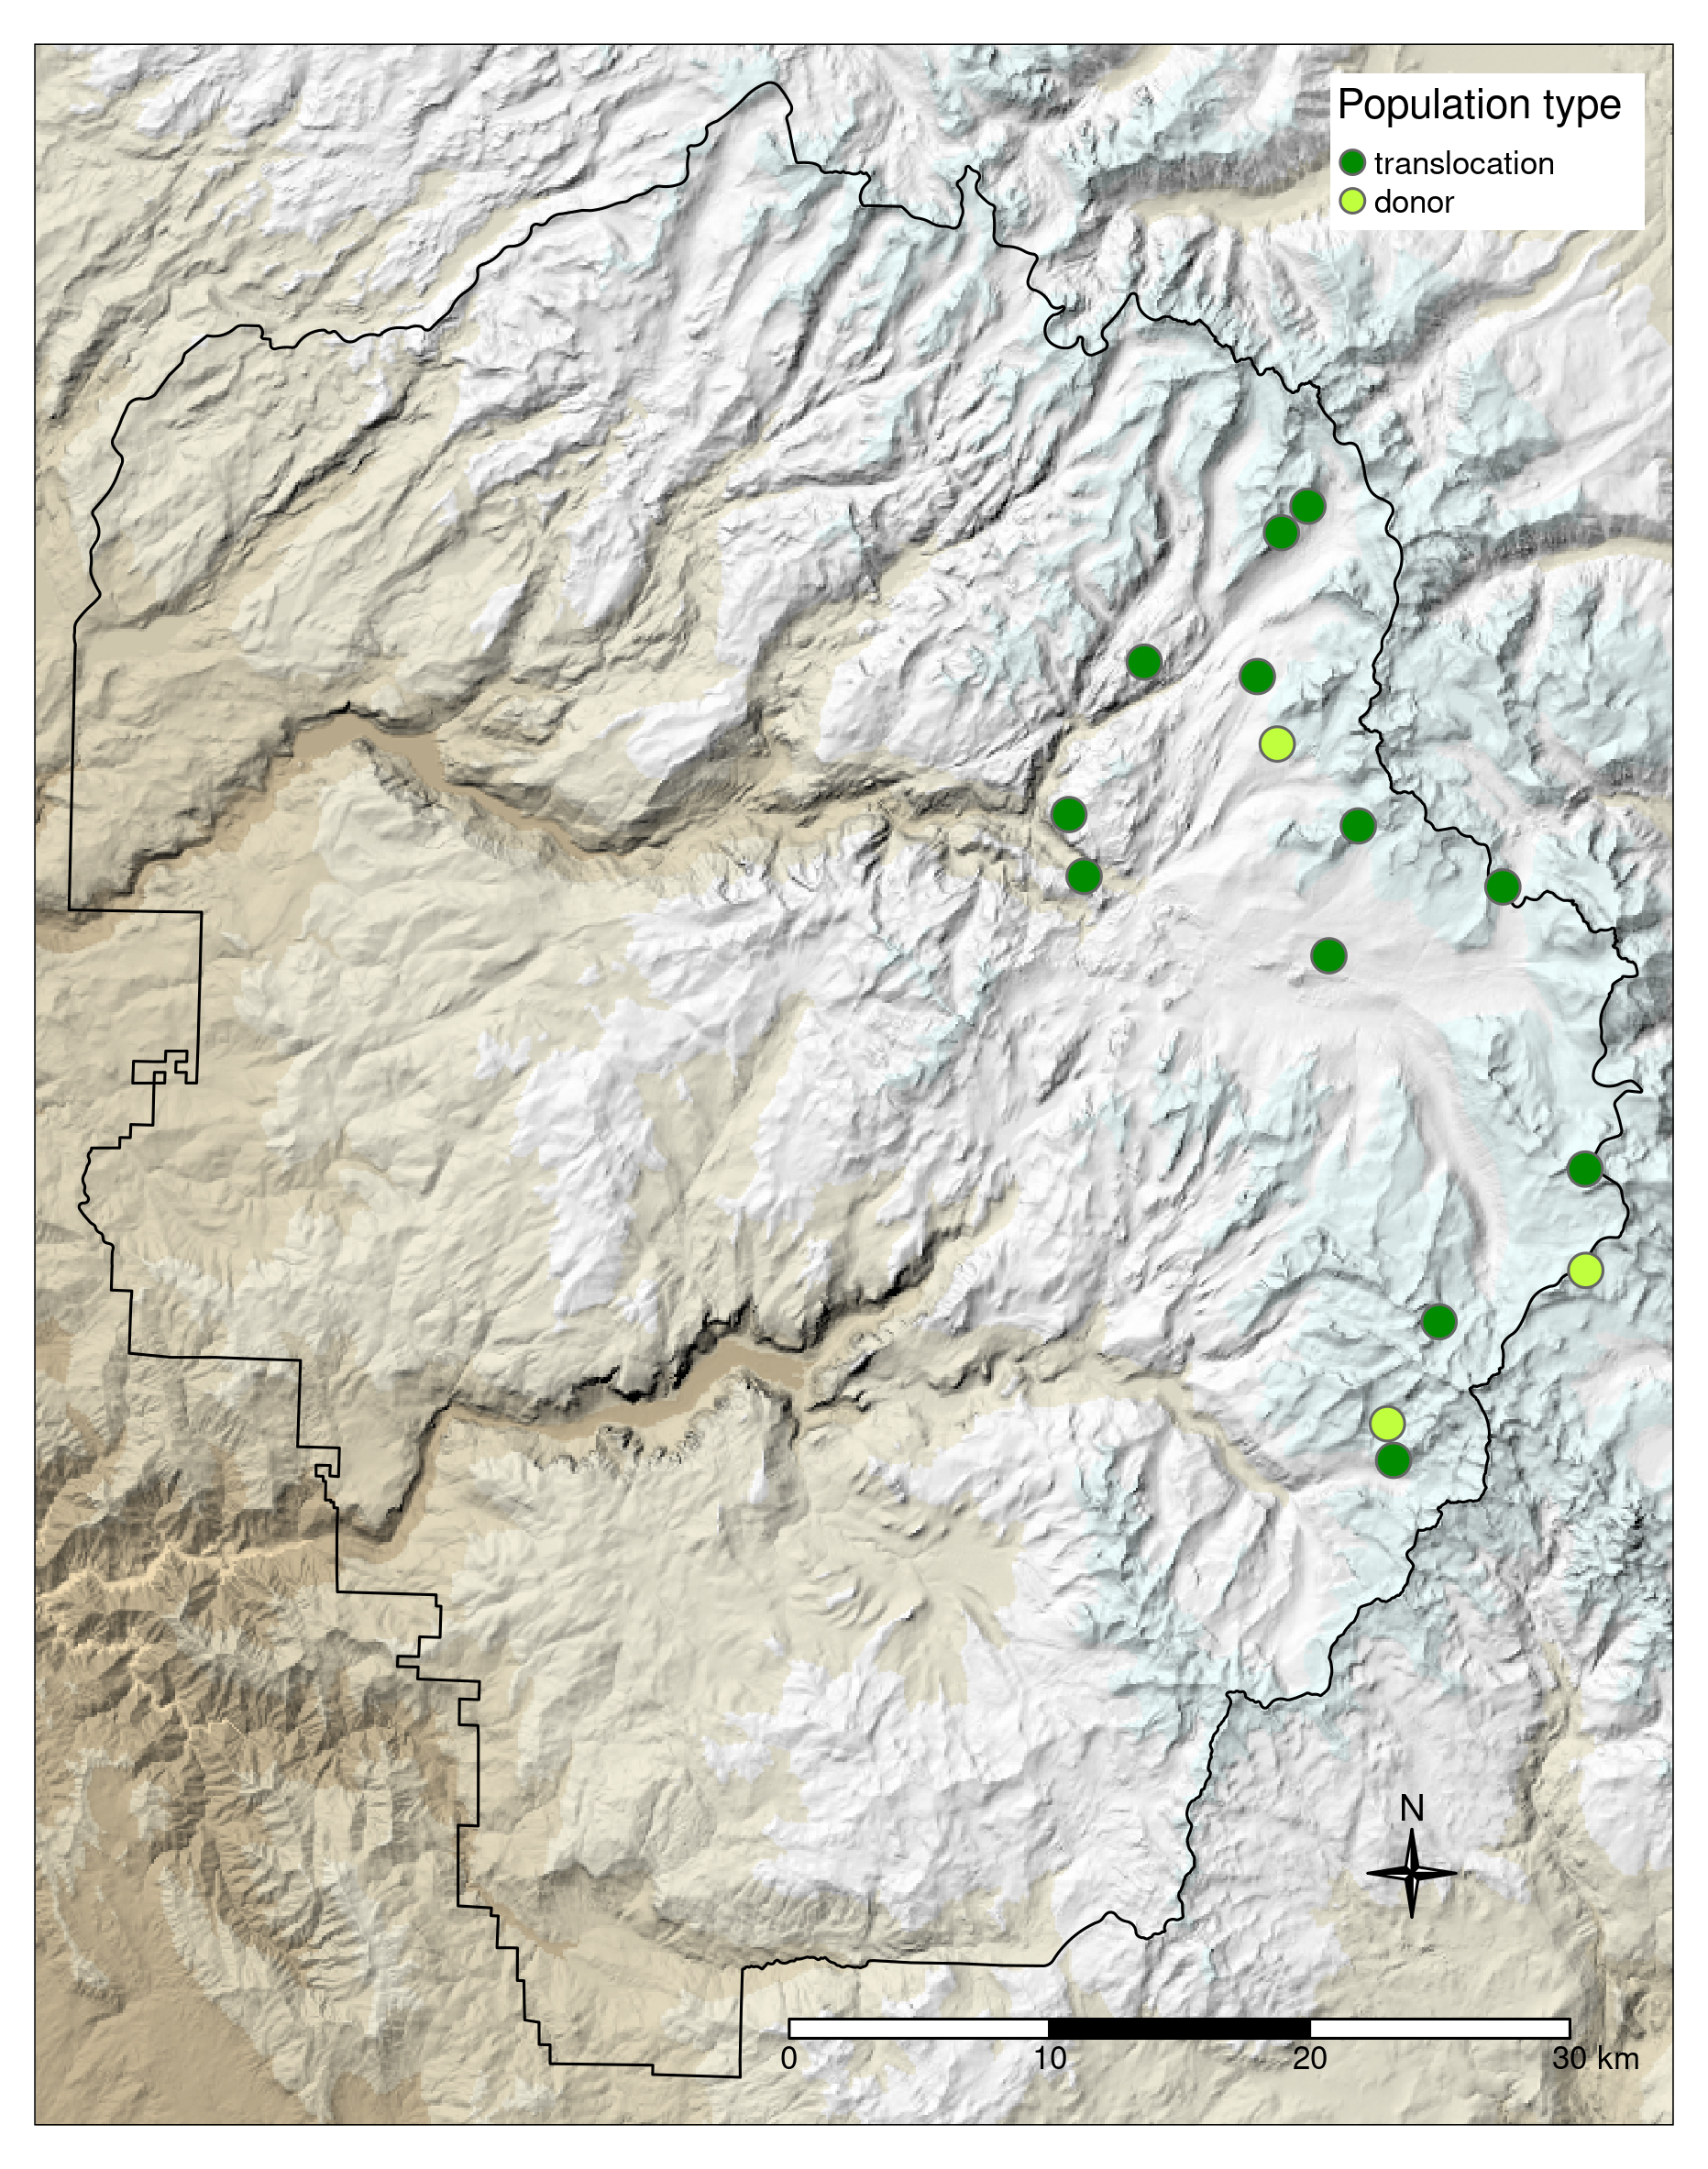
\includegraphics[width=0.60\textwidth]{figures/map_translocation_points.png}

}

\caption{\label{fig-yosemap}Map showing the locations of translocated
and donor MYL frog populations in Yosemite National Park (park boundary
indicated by gray polygon). Symbol shapes indicate the donor population
used for each translocation site, and 5-digit numbers identify each
donor and translocation site. To obscure the exact locations of
populations, random noise was added to all point coordinates. Inset map
shows the location of Yosemite within California. In both maps,
elevation is indicated by the colored hillshade layer (dark green =
lowest elevation, white = highest elevation).}

\end{figure}\clearpage

\newpage

\begin{figure}

{\centering 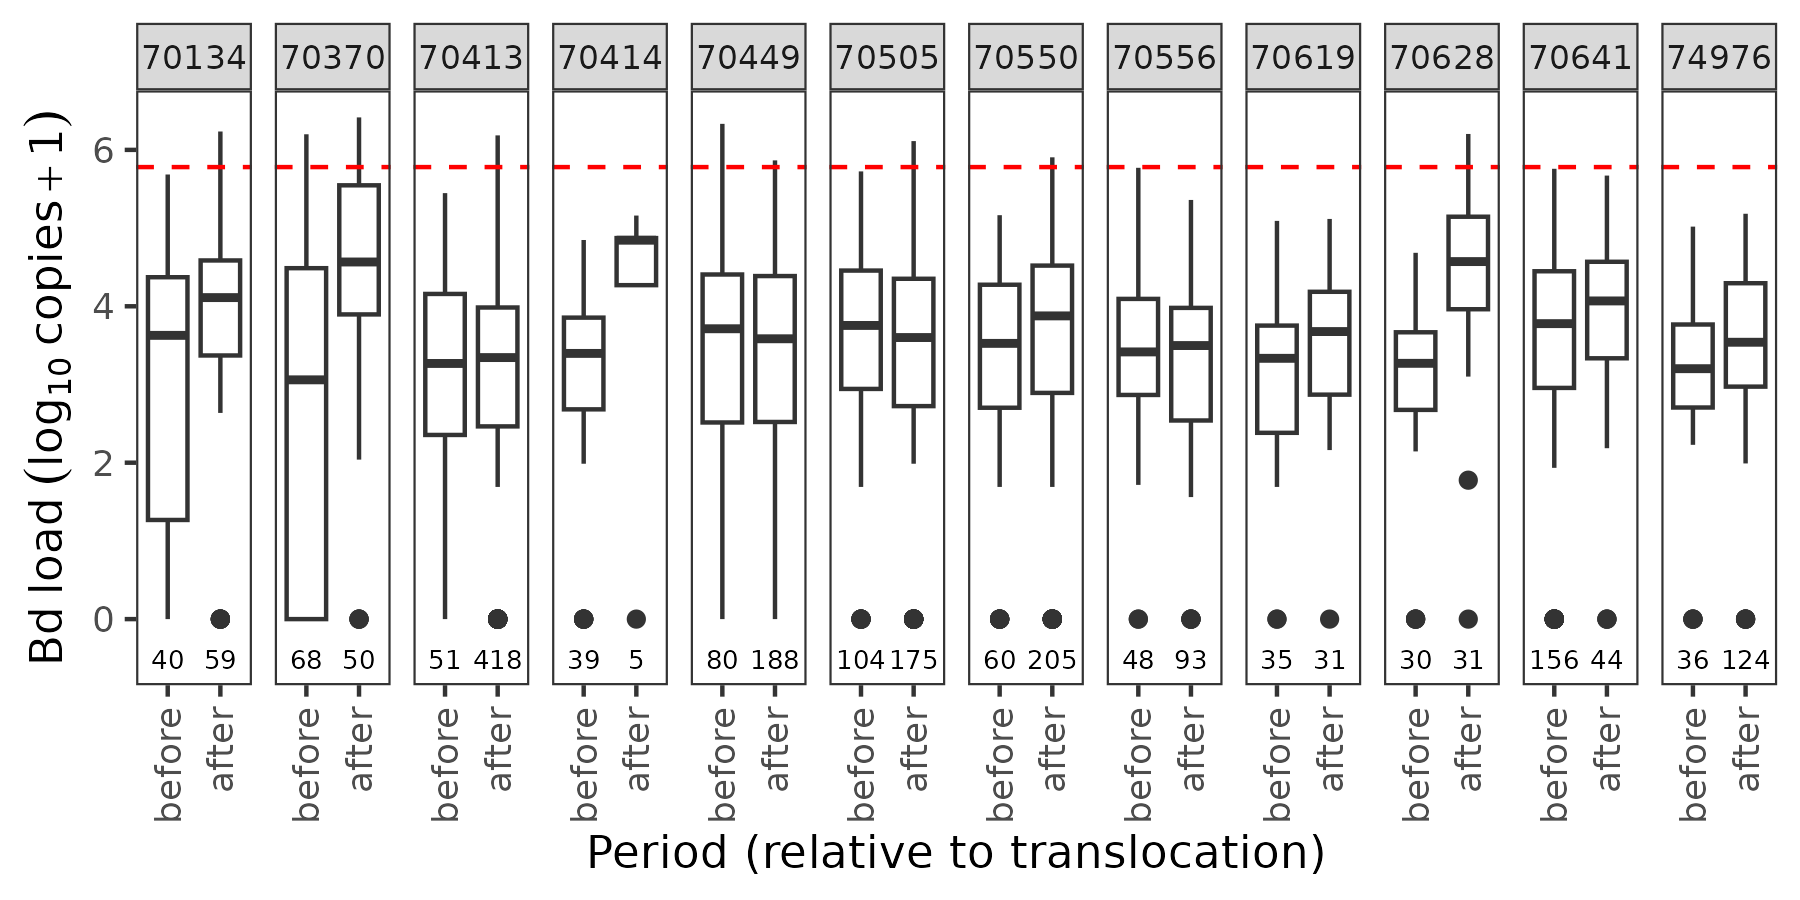
\includegraphics[width=0.7\textwidth]{figures/bdload_beforeafter.png}

}

\caption{\label{fig-bdload-beforeafter}For frogs translocated to each of
the 12 recipient sites, Bd loads for the period immediately prior to
translocation versus during the 1-year period after translocation. Bd
loads are expressed as the number of ITS1 copies per skin swab, as
estimated by qPCR of the Bd ITS1 region. Box plots show medians, first
and third quartiles, largest and smallest values within 1.5x
interquartile range, and values outside the 1.5x interquartile range.
Loads indicative of severe disease are \textgreater{} 5.8 ITS copies (on
a log\textsubscript{10} scale). Samples sizes are provided immediately
above the x-axis.}

\end{figure}\clearpage

\newpage

\begin{figure}

{\centering 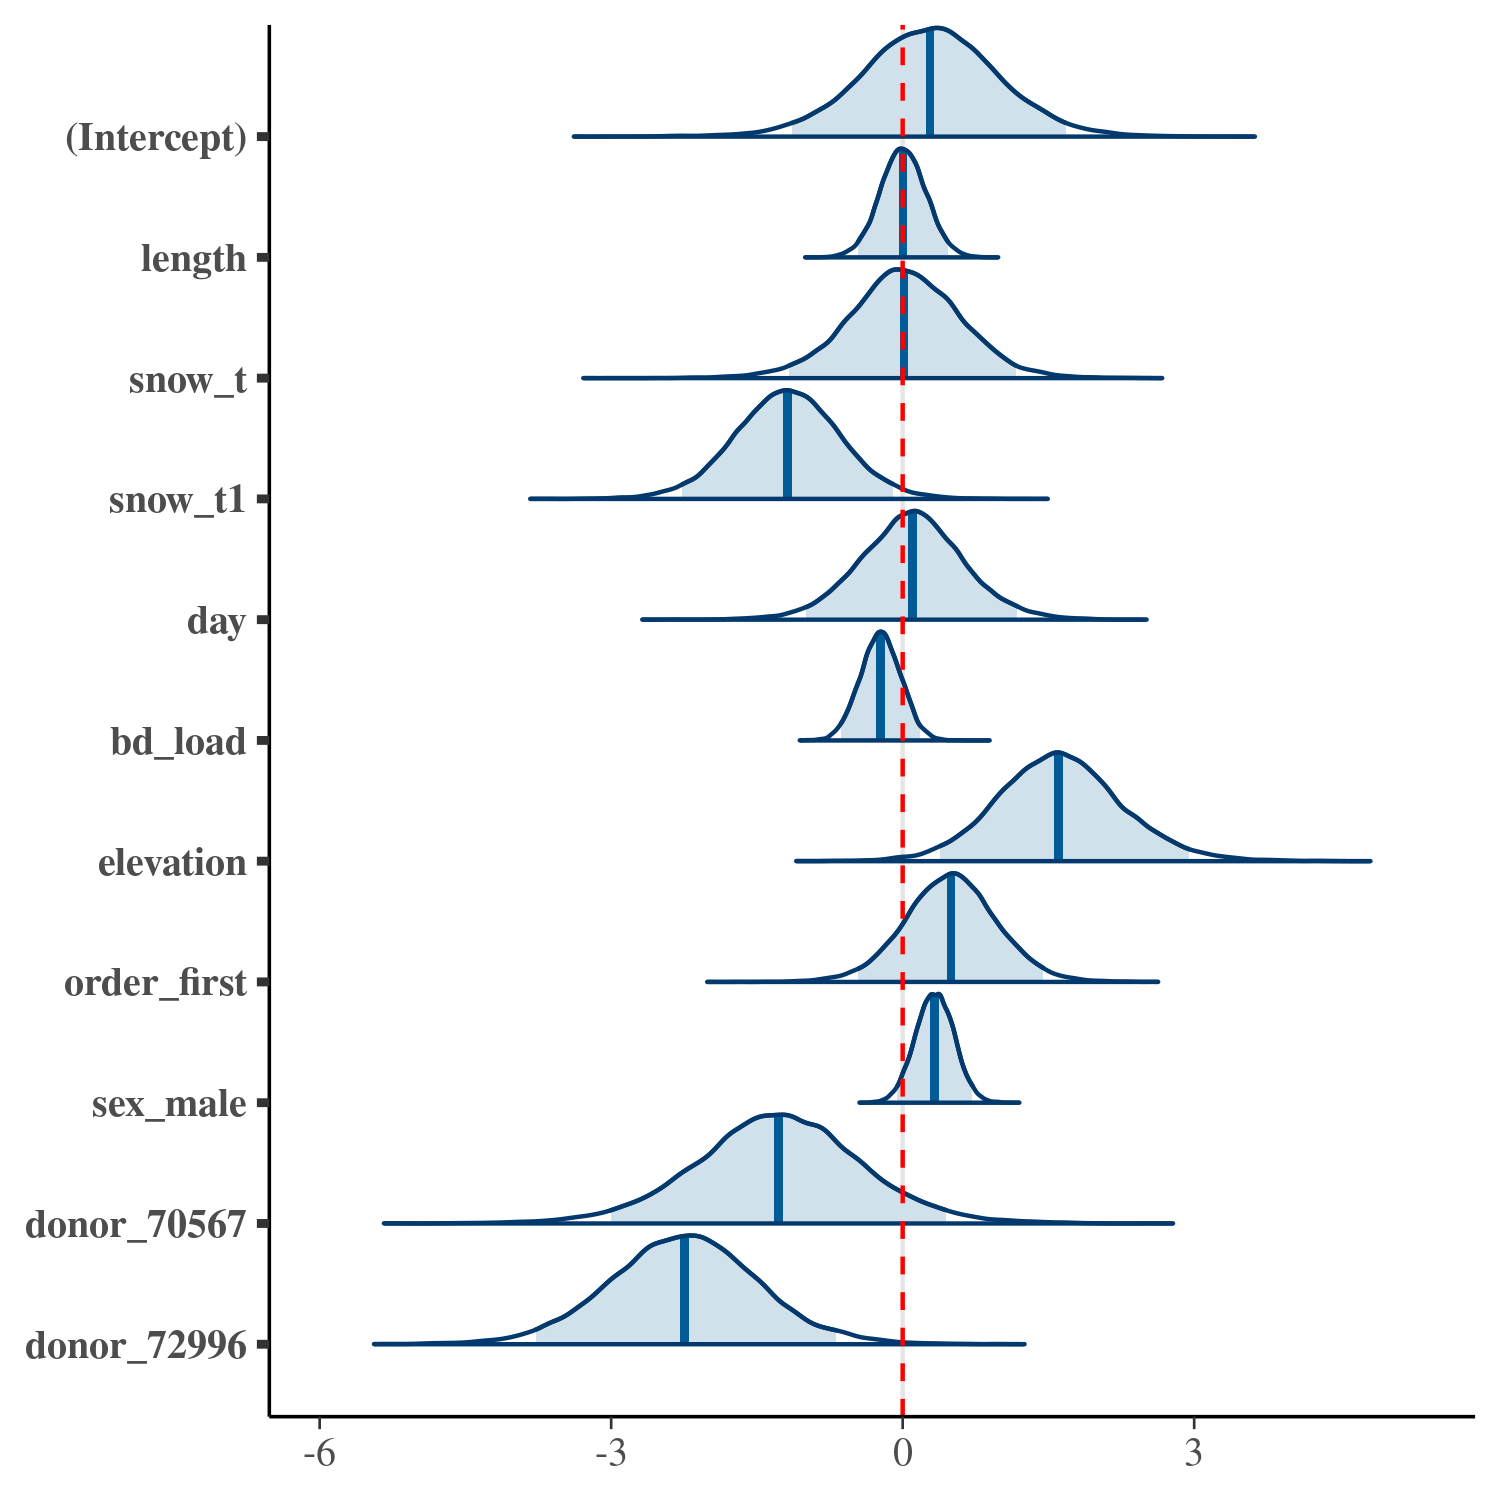
\includegraphics[width=0.60\textwidth]{figures/mcmc_areas_m1d.png}

}

\caption{\label{fig-survival-postdens}Results from the among-site
meta-analysis, showing that Bd load is not an important predictor of
post-translocation frog survival. Depicted distributions are the
estimated posterior density curves and shaded 95\% uncertainty intervals
for the intercept and all predictor variables from the best model. In
the Bayesian framework in which the model was developed, variables are
considered important predictors if the associated uncertainty interval
does not overlap zero (indicated by the dashed red line). Predictor
variables shown on the y-axis are defined as follows: length = frog
size, snow\_t = winter severity in the year of translocation (measured
on April 1), snow\_t1 = winter severity in the year following
translocation (measured on April 1), day = day of year on which a
translocation was conducted, bd\_load = Bd load, elevation = site
elevation, order\_first = within-site translocation order, sex\_male =
frog sex, donor\_70567 and donor\_72996 = donor population.}

\end{figure}\clearpage

\newpage

\begin{figure}

{\centering 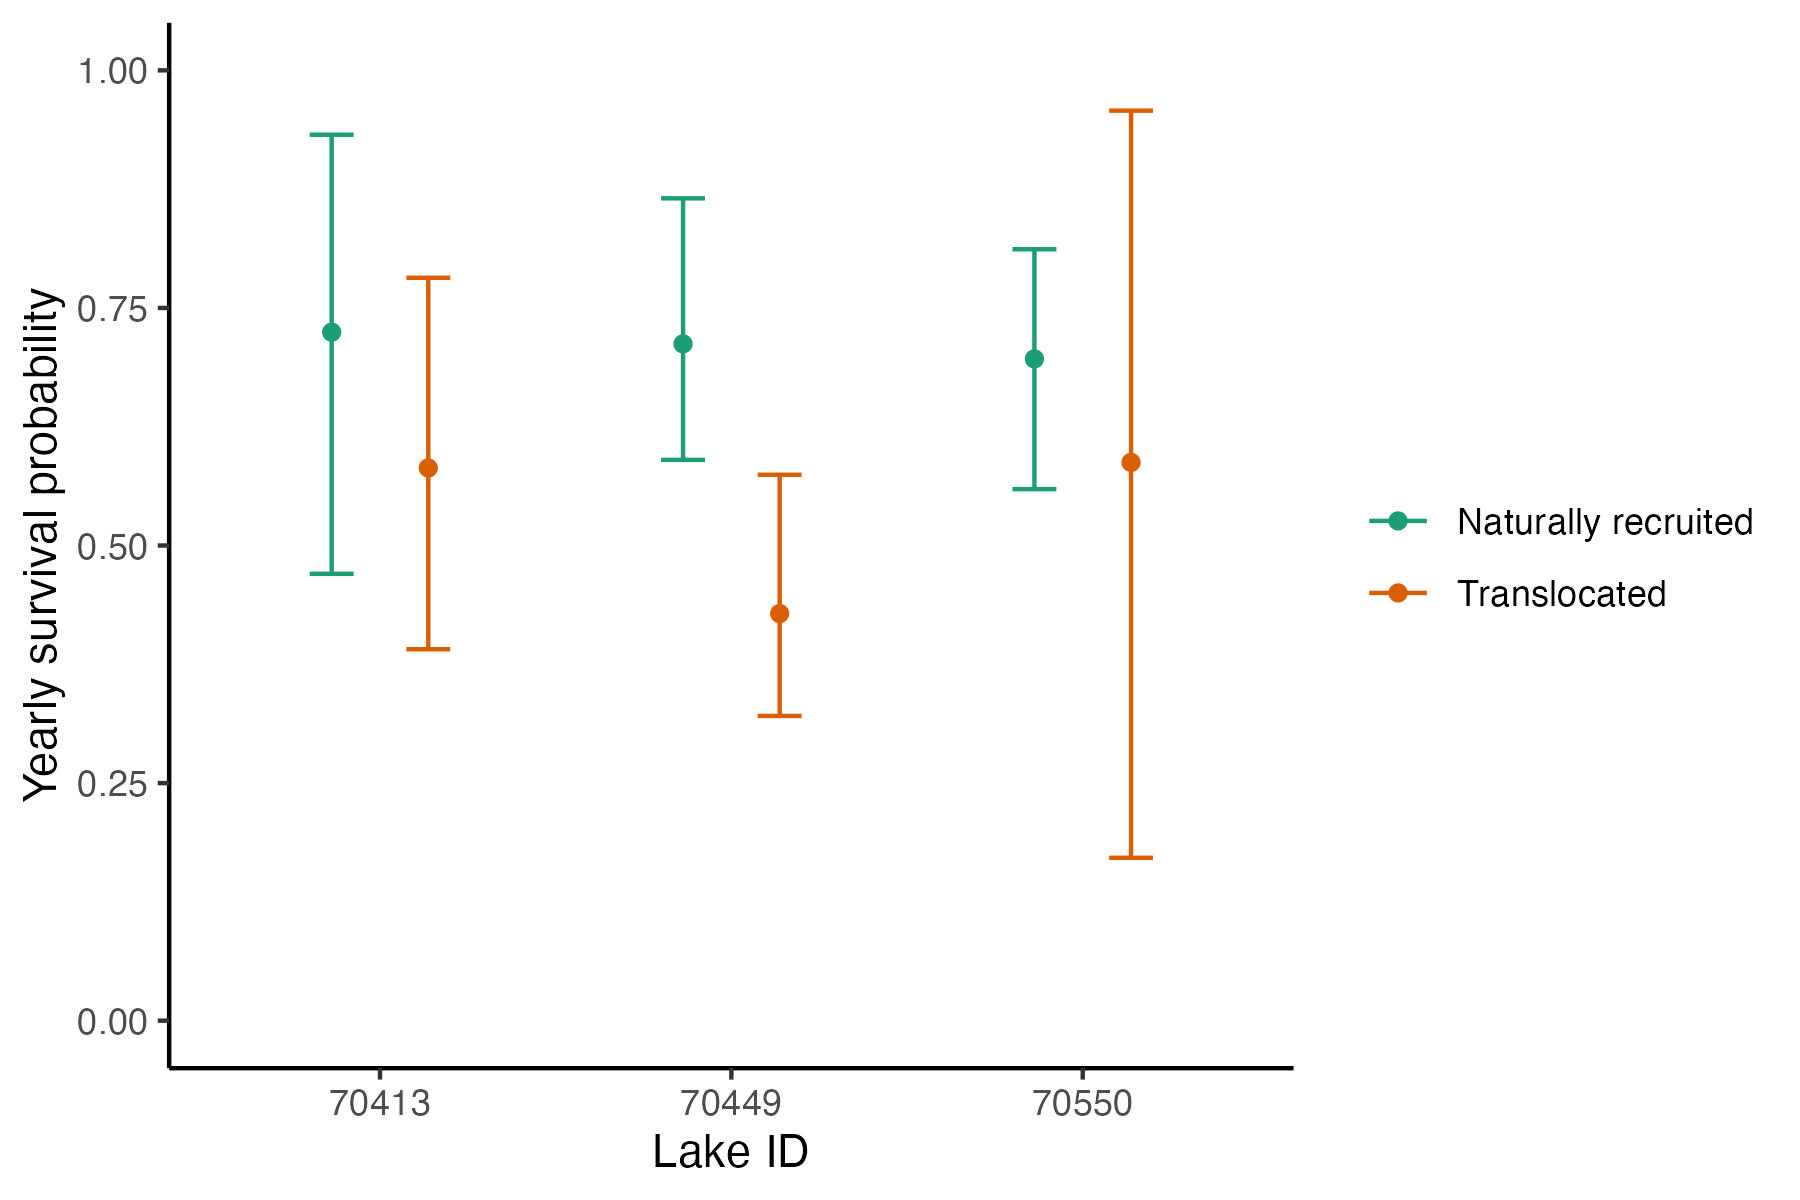
\includegraphics[width=0.60\textwidth]{figures/compare_surv_probs.jpg}

}

\caption{\label{fig-compare_surv_probs}Comparison of average yearly
adult survival probabilities for adults translocated to each of 3 sites
versus adults that were naturally recruited at each site (as a result of
reproduction by translocated frogs). In contrast to
Fig. 3, these are not survival
probabilities from the first year following translocation, but instead
represent averaged survival probabilities across multiple years and
cohorts. Points are median estimates and error bars give the 95\%
uncertainty intervals around the estimates, accounting for yearly
variation in survival probabilities. All estimates were derived using
the mrmr package, and the methods for calculation are described in
\textbf{Supporting Information - Population viability modeling --
Estimating model parameters}.}

\end{figure}\clearpage

\newpage

\begin{figure}

{\centering 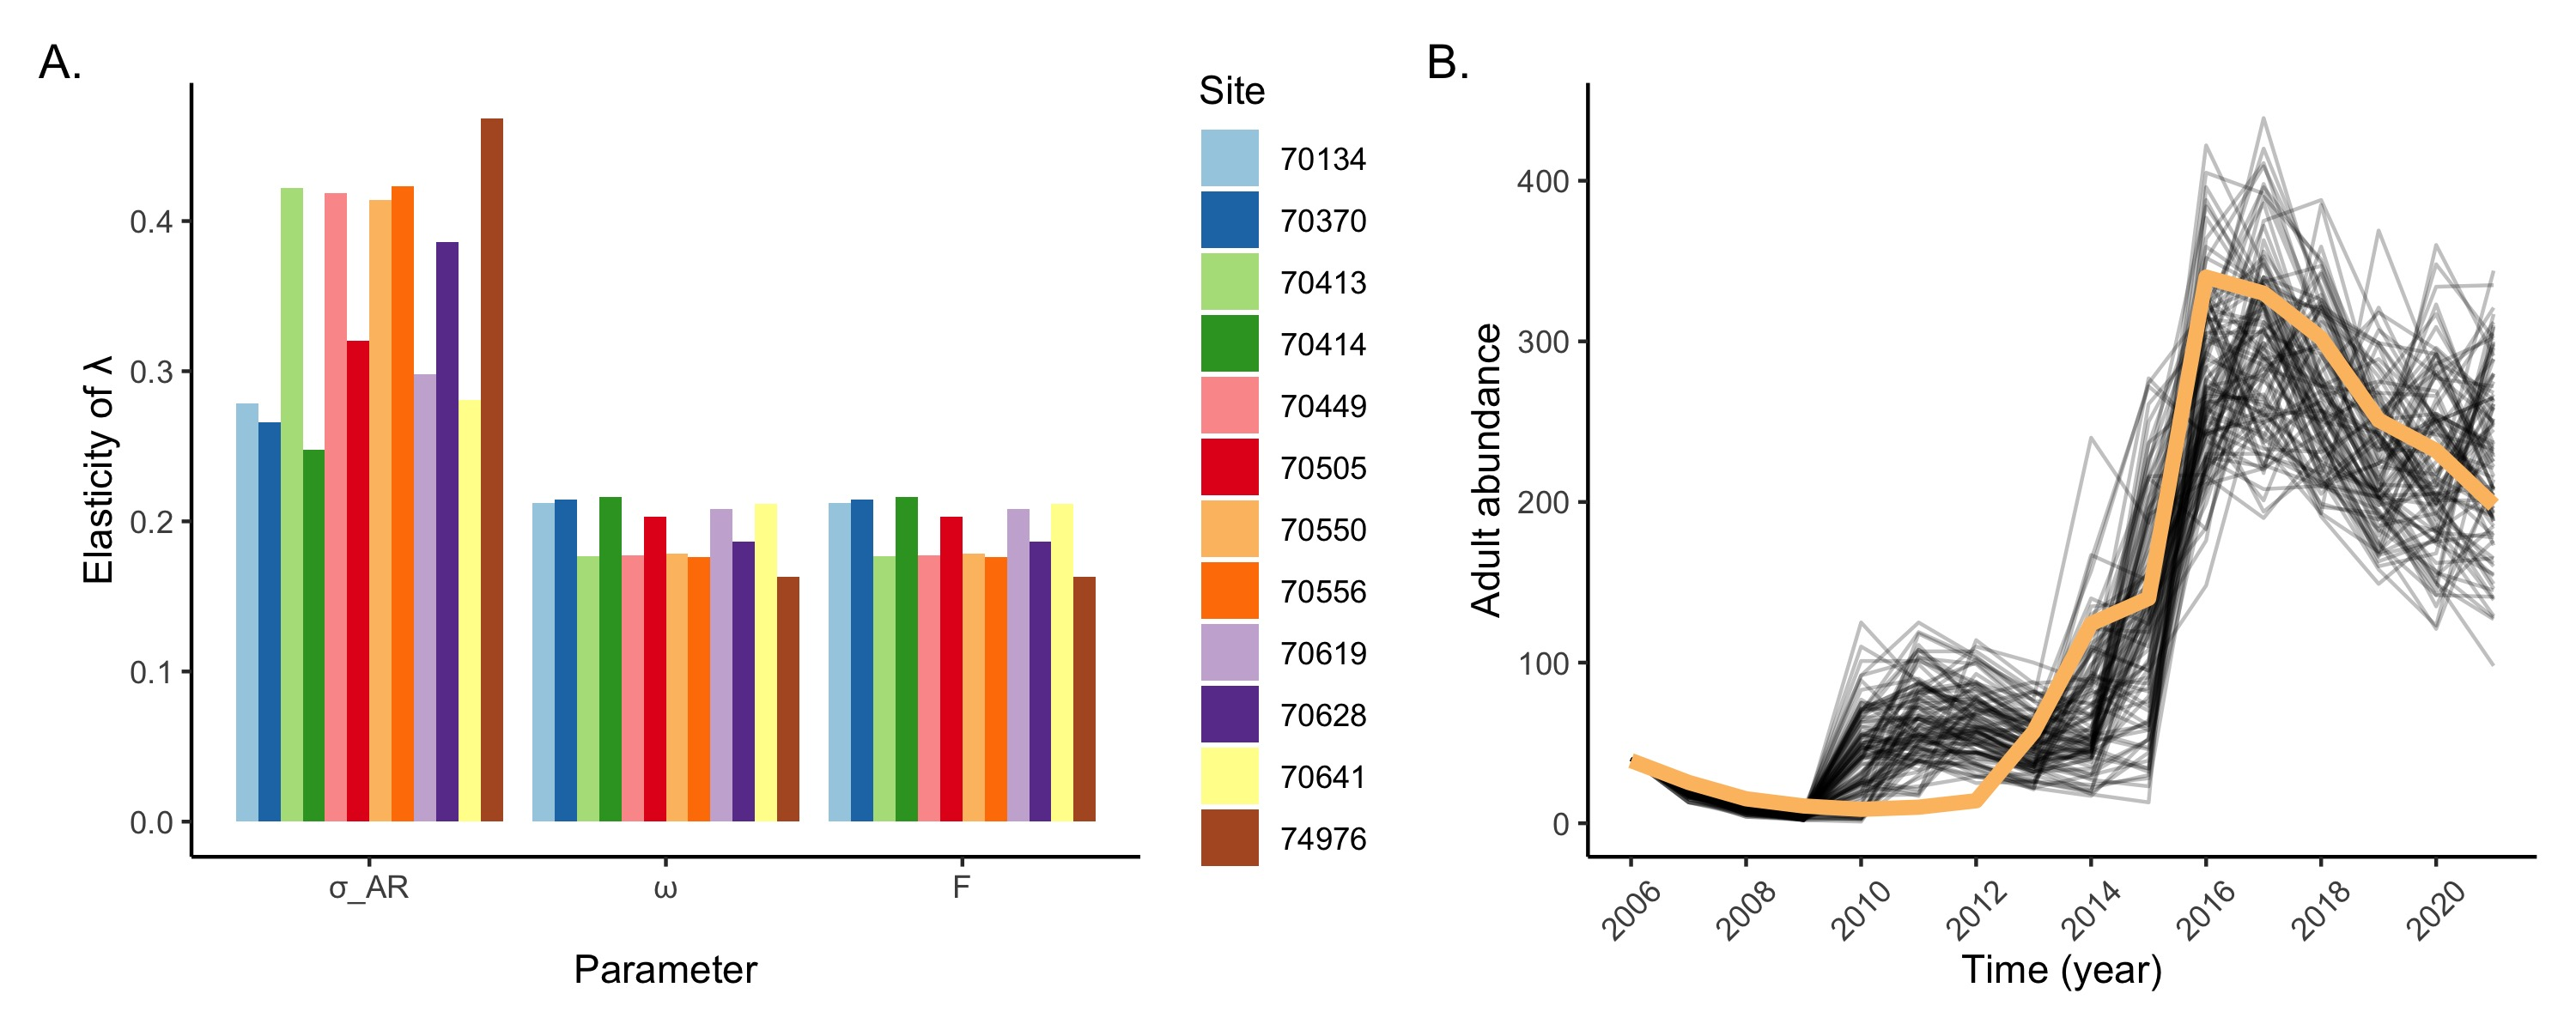
\includegraphics[width=0.60\textwidth]{figures/pop_viability_figures_for_supp.jpg}

}

\caption{\label{fig-viability-supp}Sensitivity analysis of the
stage-structured MYL frog model. Elasticity of \(\lambda\) with changes
in four parameters: \(\sigma_{A_R}\) (yearly survival probability of
naturally recruited adults), \emph{F (}number of eggs produced by a
female frog in a year that successfully hatch), \(\sigma_{J_1}\) (yearly
probability of survival of year 1 juveniles that also affects
recruitment), and \(\sigma_{J_2}\) (yearly probability of survival and
recruitment of year 2 juveniles). Elasticity is calculated at the
default parameter values for each population and \(\sigma_{J_1}\) =
0.09.}

\end{figure}\clearpage

\newpage

\begin{figure}

{\centering 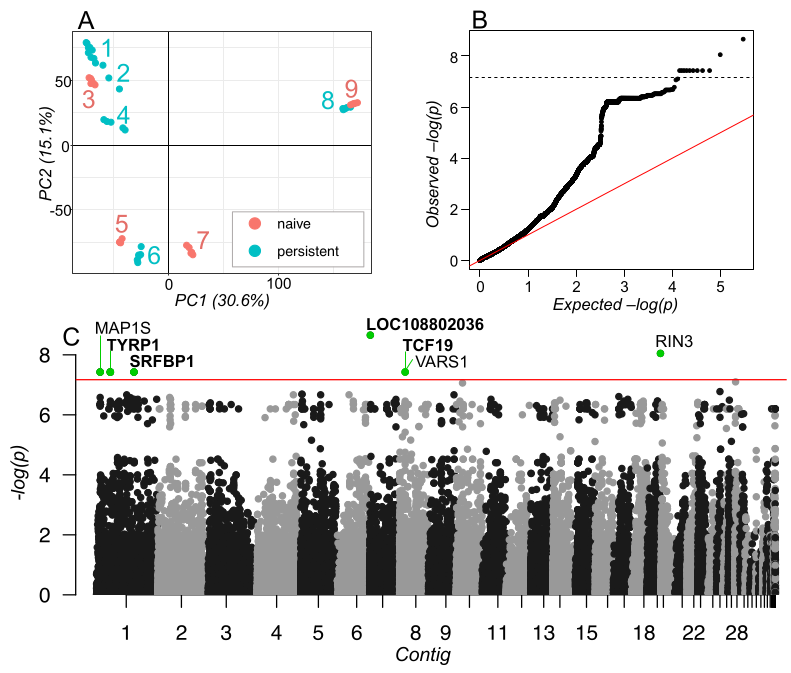
\includegraphics[width=0.85\textwidth]{figures/pca_qq_manhattan.png}

}

\caption{\label{fig-selectionresults}Results from the analysis of
individual variants, showing putative signatures of selection in
recovering MYL frog populations. (A) PCA calculated from binary SNPs
showing the genomic relationship of samples. Numeric labels and colors
match those in Fig. 1A. Populations 1-7 are
\emph{R. sierrae} and populations 8 and 9 are \emph{R. muscosa}. (B)
qqplot showing observed and expected p-values for 148,307 SNPs and
INDELS. Dashed line shows p-value that identifies outliers. (C)
Manhattan plot showing p-value for each SNP. SNPs are sorted by genomic
position and contigs are sorted by size. Red line shows p-value that
identifies outliers. Outlier SNPs above this threshold are highlighted
and labeled. Bold labels indicate the presence of at least one
non-synonymous SNP in that gene.}

\end{figure}\clearpage

\newpage

\begin{figure}

{\centering 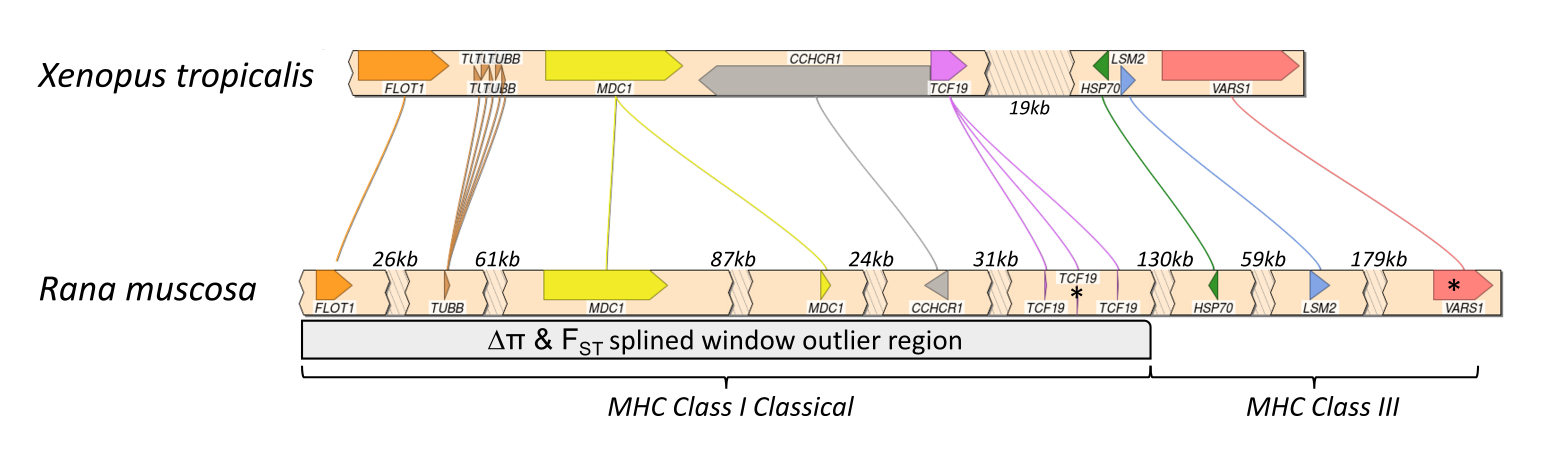
\includegraphics[width=0.85\textwidth]{figures/synteny_figure.png}

}

\caption{\label{fig-synteny-plot}Synteny plot showing conserved gene
order in \emph{Xenopus tropicalis} and \emph{Rana muscosa} for the
outlier region containing MHC Class I Classical and MHC Class III gene
regions. The plot was created with SimpleSynteny (95) using
\emph{Xenopus tropicalis} Chromosome 8 (NC\_030684.2, genbank accession
GCA\_000004195.4) and \emph{Rana muscosa} Contig19. Asterices indicate
the location of SNP outliers in the TCF19 and VARS1 genes. Gap sizes for
each contig representation are labeled.}

\end{figure}\clearpage

\newpage

\begin{figure}

{\centering 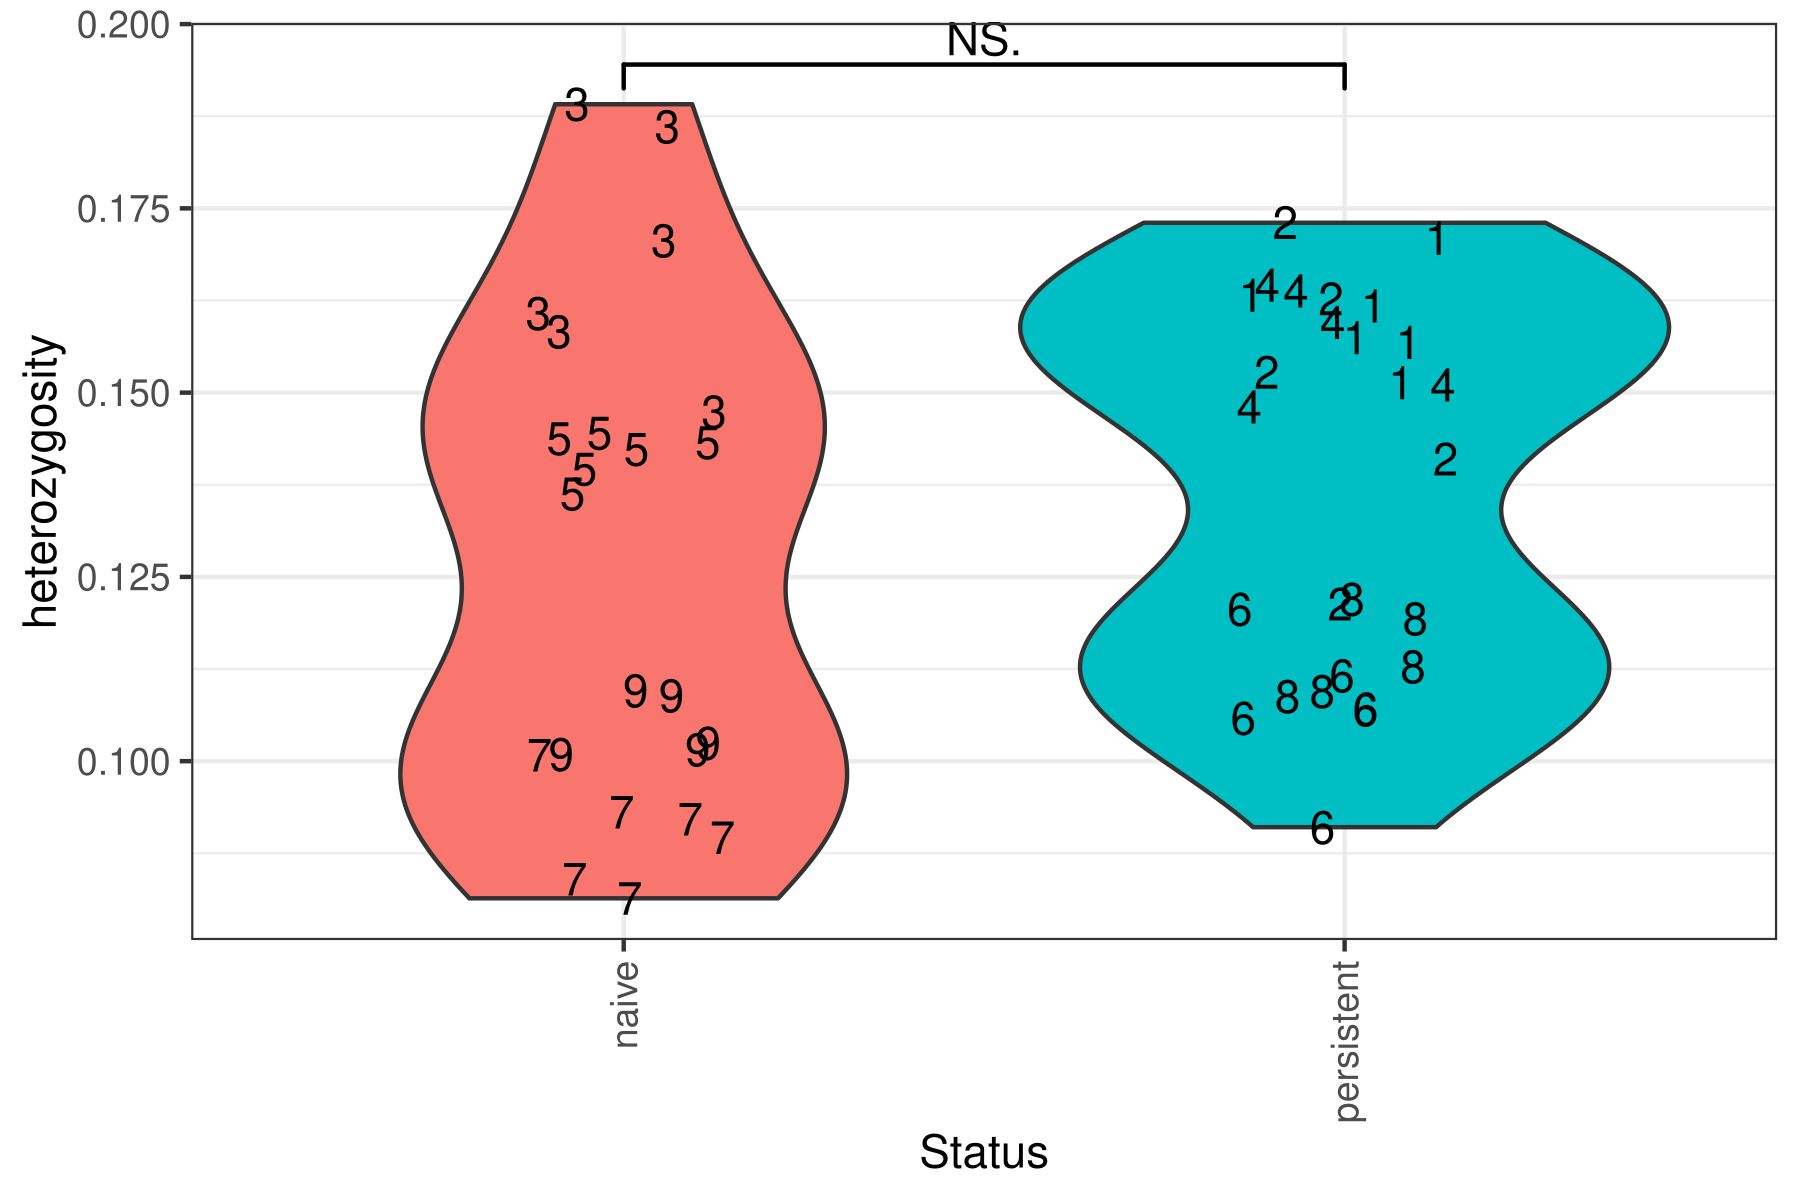
\includegraphics[width=0.85\textwidth]{figures/het_by_status_violin_plot.png}

}

\caption{\label{fig-violinplot-heterozy}Violin plots showing individual
heterozygosity for the Bd-naive and recovering populations included in
the frog evolution study. Individual data points are represented by
their corresponding site number (from
Fig. 1). A Wilcoxon signed-rank test showed
no significant difference between the two groups.}

\end{figure}\clearpage

\newpage

\begin{figure}

{\centering 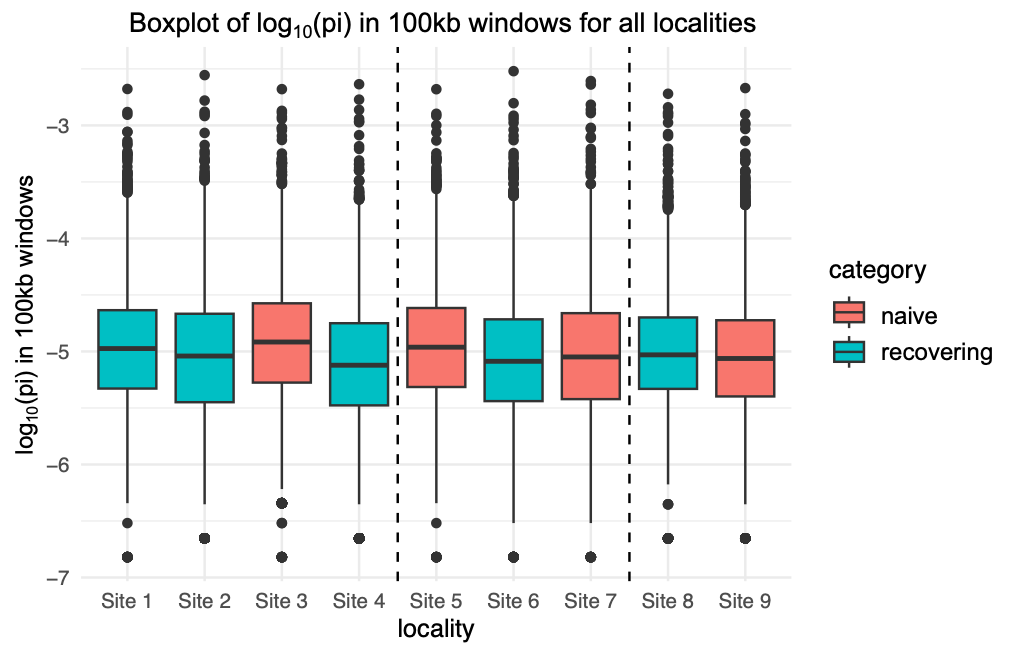
\includegraphics[width=0.85\textwidth]{figures/boxplot_pi_by_site.png}

}

\caption{\label{fig-boxplot-pi}For each study population in the frog
evolution study (from Fig. 1), boxplots
showing nucleotide diversity (\(\pi\)) within 100kb sliding windows
along the genome. The y-axis has been log\textsubscript{10}-transformed
for display purposes. Sites are color-coded as ``Bd-naive'' or
``recovering'', and vertical dashed lines show the genetic breaks
between frog populations as described in
Figure~\ref{fig-selectionresults} A). Within the genetic clusters,
mean \(\pi\) is significantly different between sites (p \textless0.001
Wilcoxon rank-sum test).}

\end{figure}\clearpage

\newpage

\begin{figure}

{\centering 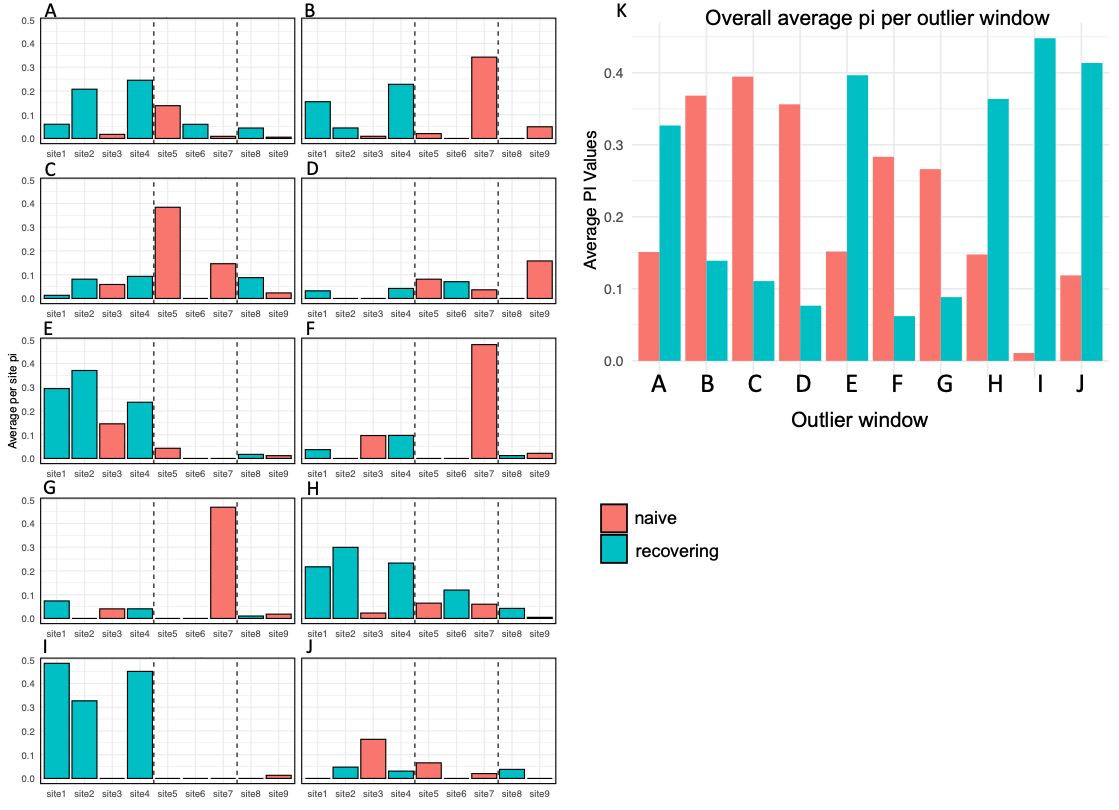
\includegraphics[width=0.85\textwidth]{figures/perwindow_persite_pi.png}

}

\caption{\label{fig-barchart-pi-by-windowsite}For each study population
in the frog evolution study, average \(\pi\) values by population
calculated for each of the 10 outlier windows identified in the splined
window analysis (A-J). Sites are color-coded as ``Bd-naive'' or
``recovering'', and vertical dashed lines show the genetic breaks
between frog populations as described in
Figure~\ref{fig-selectionresults} A. Gene annotations for the outlier
regions are as follows: (A) C6, C7, (B) DDX10, ZBTB24, (C) SULTR-like,
TRAF3IP2, VGLL3, EXOC1, (D) FLOT1, TUBB2B, TUBB, MDC1, CCHCR1,
TCF19\emph{, TRIM29, HSP70, LSM2, VARS,} (E) GCC2, CFAP251, PEG10, (F)
ERO1A, GVINP1, (G) ERO1A, GVINP1, (H) PPP1R12A, TSPAN4, PAWR, MFRP, MAX,
PPP6R3, (I) C6H5ORF22, PKS6, BSPRY, MPV17, and (J) CAD, ATRAID, GPN1.
Note that windows F and G are in the same gene region. * by gene names
indicate that an outlier SNP is also present in this gene . (K) Average
\(\pi\) values of naive and recovering groups for each of the outlier
windows shown in A-J. }

\end{figure}\clearpage

\newpage

\hypertarget{tables}{%
\subsubsection{Tables}\label{tables}}

\hypertarget{tbl-param_values}{}
\begin{longtable}[]{@{}
  >{\raggedright\arraybackslash}p{(\columnwidth - 4\tabcolsep) * \real{0.3611}}
  >{\raggedright\arraybackslash}p{(\columnwidth - 4\tabcolsep) * \real{0.2639}}
  >{\raggedright\arraybackslash}p{(\columnwidth - 4\tabcolsep) * \real{0.3750}}@{}}
\caption{\label{tbl-param_values}Description and values of parameters
used in the model. All survival probabilities are in the presence of the
fungal pathogen Bd.}\tabularnewline
\toprule()
\begin{minipage}[b]{\linewidth}\raggedright
\textbf{Parameter}
\end{minipage} & \begin{minipage}[b]{\linewidth}\raggedright
\textbf{Value}
\end{minipage} & \begin{minipage}[b]{\linewidth}\raggedright
\textbf{Source}
\end{minipage} \\
\midrule()
\endfirsthead
\toprule()
\begin{minipage}[b]{\linewidth}\raggedright
\textbf{Parameter}
\end{minipage} & \begin{minipage}[b]{\linewidth}\raggedright
\textbf{Value}
\end{minipage} & \begin{minipage}[b]{\linewidth}\raggedright
\textbf{Source}
\end{minipage} \\
\midrule()
\endhead
\(\sigma_{L_1}\), Yearly survival probability of year 1 tadpoles & 0.7 &
Estimated from field data, observations, natural history knowledge \\
\(\sigma_{L_2}\), Yearly survival probability of year 2 tadpoles & 0.7 &
Estimated from field data, observations, natural history knowledge \\
\(\sigma_{L_3}\), Yearly survival probability of year 3 tadpoles & 0.7 &
Estimated from field data, observations, natural history knowledge \\
\(\sigma_{J_1}\), Yearly survival probability of year 1 juveniles &
Varies yearly & Varies. Bounds estimated from field data, observations,
natural history knowledge \\
\(\sigma_{J_2}\), Yearly survival probability of year 2 juveniles & 0.5
& Estimated from field data, observations, natural history knowledge \\
\(\sigma_{A_R}\), Yearly survival probability of naturally recruited
adults & Varies by population & Estimated from CMR studies \\
\(\sigma_{A_T}\), Yearly survival probability of translocated adults &
Varies by population & Estimated from CMR studies \\
\(p_{L_1}\), Probability of a year 1 tadpoles remaining as a tadpoles &
1 & Estimated from field data, observations, natural history
knowledge \\
\(p_{L_2}\), Probability of a year 2 tadpoles remaining as a tadpoles &
0.25 & Estimated from field data, observations, natural history
knowledge \\
\(p_{J_1}\), Probability of a year 1 juvenile remaining as a juvenile &
0.25 & Estimated from field data, observations, natural history
knowledge \\
\(p_F\), Probability of a adult female reproducing in a year & 0.5 &
Could be as high at 1, based on field observations \\
\(F\), Number of surviving eggs produced by an adult female & 100 & From
observations of captive frogs \\
\bottomrule()
\end{longtable}

\newpage


%%% Add this line AFTER all your figures and tables
\FloatBarrier

\dataset{gemma\_outliers\_all.csv}{Set of liberal SNP and INDEL outlier variants (Bonferroni corrected p-value $<$ 0.05), identified via GEMMA.}

\dataset{gemma\_outliers\_strict\_freq.csv}{Set of strict SNP and INDEL outlier variants (Bonferroni corrected p-value $<$ 0.01), identified via GEMMA.
Additional information includes variant location within the gene (predicted\_gene\_loc) and whether the variant is synonymous or nonsynonymous (predicted\_effect\_AA).}

\dataset{spline\_window\_shared\_outliers.csv}{Description of overlapping \emph{F\textsubscript{ST}} and
\(\pi_{diff}\) outlier windows, as identified in the splined window
analysis.}

\dataset{spline\_window\_gene\_details.csv}{Annotation information for all genes within each of the
overlapping outlier windows in dataset S3}

\bibliography{translocation}

\end{document}

